\section{AGO70}
The space debris images are acquired using astronomical telescopes. 
In our thesis, we are working with images captured at the Astronomical and Geophysical Observatory (AGO) in Modra. The acquisition of images at AGO is performed by the reflecting Newtonian telescope (AGO70) \cite{ago702018}, shown in the Figure \ref{img:ago70}. 

\begin{figure}[h]
    \centering
    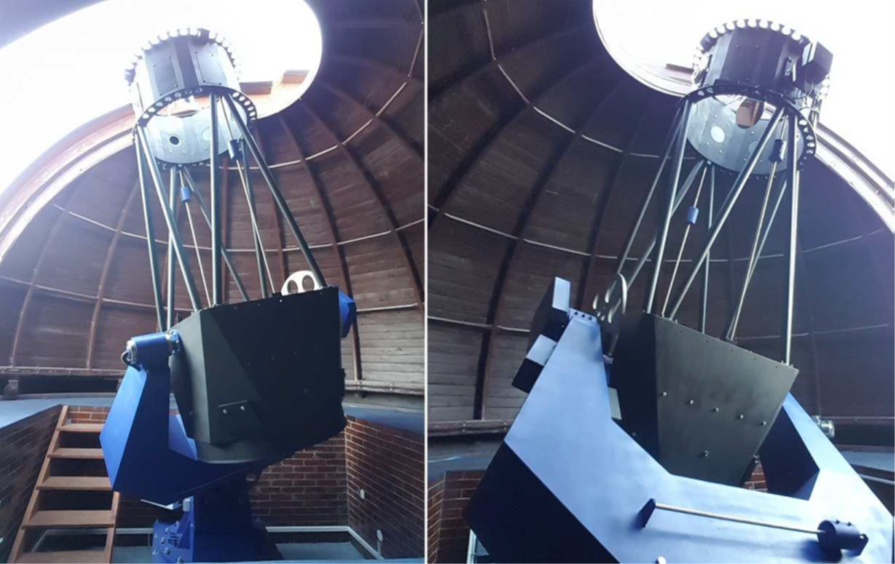
\includegraphics[width=.5\textwidth]{images/ago70.png}
    \caption{The telescope AGO70 in Modra. Source: \cite{ago702018}.}
    \label{img:ago70}
\end{figure}

In 2016, after Slovakia became the 9th member of the ESA Plan for the European Cooperating States (PECS), a contract with the Faculty of Mathematics, Physics, and Informatics (FMPI) was signed. The first action was to transform the telescope in AGO from an amateur observation tool into a professional optical system used for regular tracking of space debris. Some examples of images acquired from the space debris observations performed by AGO70 are shown in the Figure \ref{fig:ago70images}. The installation of AGO70 finished in 2016 and the telescope has the following parameters: 

\begin{itemize}
    \item 700 mm primary parabolic mirror
    \item gravity actuator supporting the parabolic mirror
    \item focal length of 2962 mm
    \item FLI Proline PL1001 Grade 1 CCD camera
    \item 24 $\mu$m pixel size of the CCD camera
    \item resolution 1024x1024
    \item 28.5' x 28.5' field of view
    \item 16 bit per pixel images
\end{itemize}


\begin{figure}[!h]
    \begin{subfigure}{.3\textwidth}
        \centering
        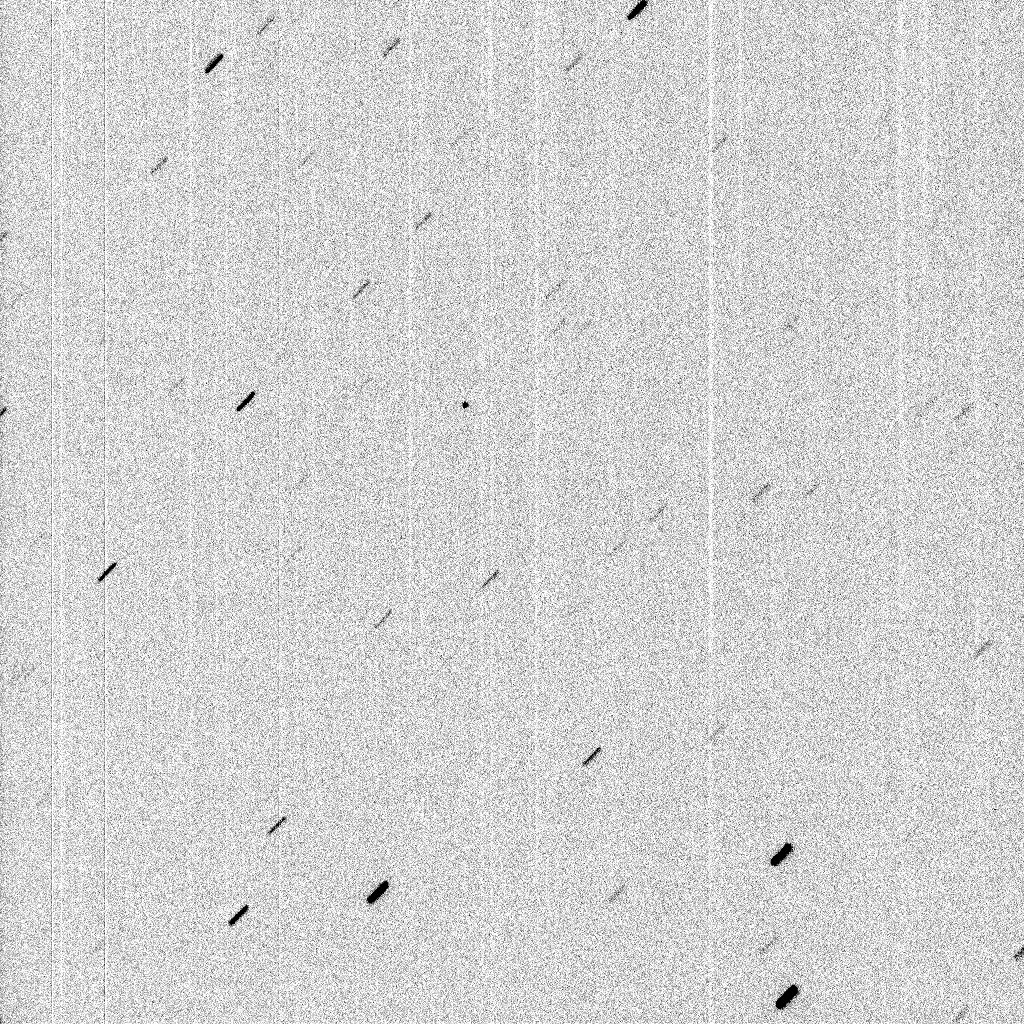
\includegraphics[width=\textwidth]{images/StreakPoint00.jpg}
    \end{subfigure}
    \hfill
    \begin{subfigure}{.3\textwidth}
        \centering
        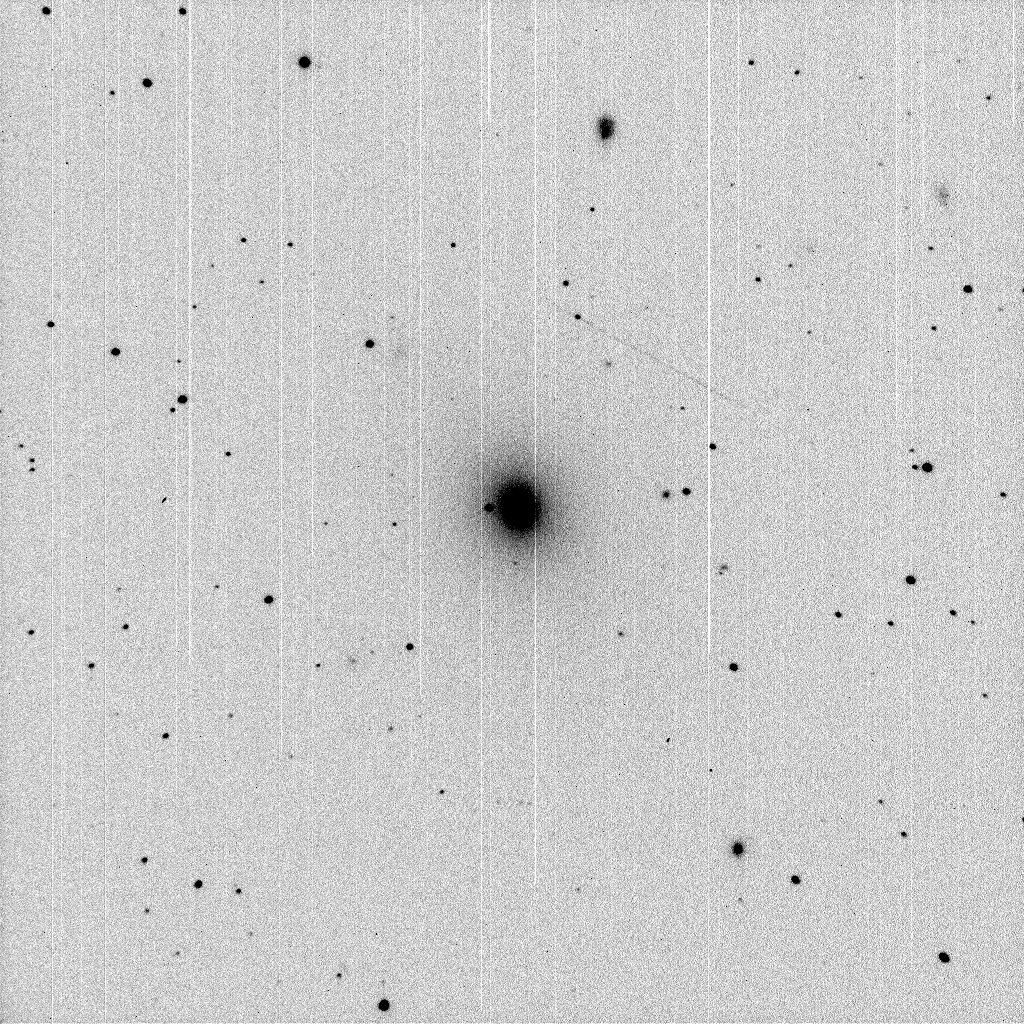
\includegraphics[width=\textwidth]{images/galaxypoints.jpg}
    \end{subfigure}
    \hfill
    \begin{subfigure}{.3\textwidth}
        \centering
        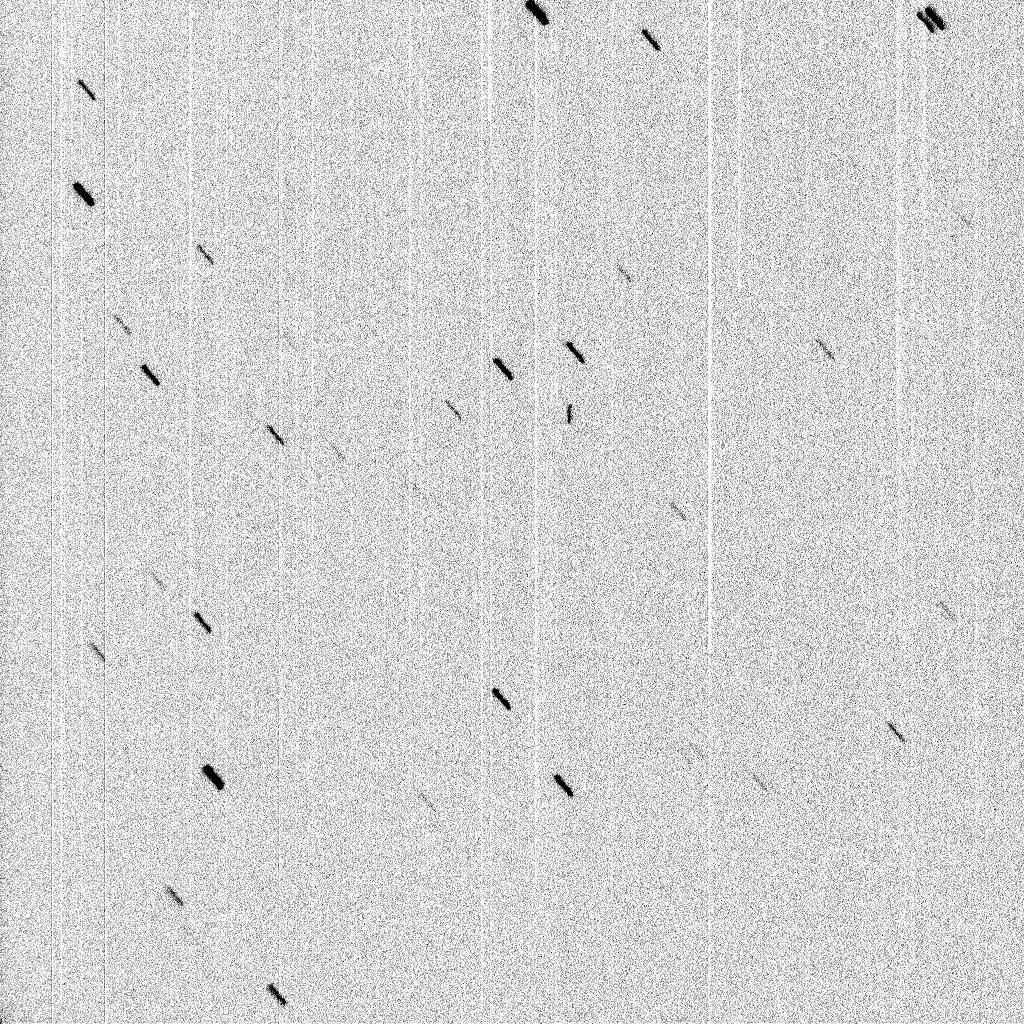
\includegraphics[width=\textwidth]{images/StreakStreak2.jpg}
    \end{subfigure}
    \hfill
    \caption{Examples of some images acquired by AGO70. }
    \label{fig:ago70images}
\end{figure}


%AGO70 has a very thin 700 mm primary parabolic mirror, which is supported by the gravity actuator. The mirror is placed at a focal length of 2962 mm. The telescope is equipped with FLI Proline PL1001 Grade 1 CCD camera and has a 28.5' x 28.5' field of view. Acquired images have a resolution of 1024x1024 pixels and contain values ranging from 0 to 65 535. 
